\section*{Systemtheorie der Sinnesorgane}
\setcounter{subsection}{3} 
\subsection{Übung}
\subsubsection{Signaladdition}
In dieser Aufgabe wurden zwei sinusförmige Signale mit den Frequenzen $f_1\ =\ \SI{400}{\Hz}$ und $f_2\ =\ \SI{404}{\Hz}$ addiert. In der Ausgabe des Tonsignales lassen sich aber nicht zwei spezifische Frequenzen unterscheiden. Man hört nur einen lauter und leiser werdenden Ton.
Dies erklärt sich folgendermaßen: Durch den geringen Frequenzunterschied kommt es nach einer konstruktiven Interferenz bei Nullphase zu einem De-Phasing (Fig. \ref{fig:signal}, Oben) und schließlich einer destruktiven Interferenz (Fig. \ref{fig:signal}, Mitte). Danach Re-Phased das Signal wieder zu einer konstruktiven Interferenz am Periodenende (Fig. \ref{fig:signal}, Unten).

Die aus den Interferenzen resultierende Schwebung bzw. Hüllkurve lässt sich mit einer Umformung durch eine Identität aus den Additionstheoremen leicht mathematisch darstellen:
\begin{align}
\omega &= 2\pi f\\
\mathrm{Seien:}&\\
y_1(t)\ =\ \sin(\omega_1 t)\ &\mathrm{und}\ y_2(t)\ =\ \sin(\omega_2 t)\\
y(t)\ &=\ y_1(t)\ +\ y_2(t) \\
&=\ \sin(\omega_1 t)\ +\ \sin(\omega_2 t)\\
&=\ 2\ \cdot\ \sin \ \left( 2 \pi \left( \frac{f_1 + f_2}{2} \right) t \right)\ \cdot\ \cos \ \left( 2 \pi \left( \frac{|f_1 - f_2|}{2} \right) t \right)\\
f_\mathrm{Schwebung}\ &=\ \left| f_1 - f_2 \right|\\
f_\mathrm{Mittelwert}\ &=\ \frac{f_1 + f_2}{2}
\end{align}

\begin{equation}
\boxed{ y(t)\ &=\ 2  \sin \! \left( 2 \pi f_\mathrm{Mittelwert} \, t \right) \cdot \cos \! \left( \pi f_\mathrm{Schwebung} \, t \right) \label{eq:schwebung}}
\end{equation}
Wie in der finalen Umformung Eq. \ref{eq:schwebung} dargestellt, ergibt sich die Addition zweier Sinusschwingungen, deren Frequenzabstand unter der Hörschwelle von \SI{20}{\Hz} liegt, zu einem Ton aus dem Mittelwert beider Summanden, der mit der Schwebungsfrequenz amplitudenmoduliert ist.

Das überlagerte Signal einer Periode ist in Figure \ref{fig:signal_super}\protect\subref{fig:signal_addition} dargestellt. Durch den Frequenzunterschied $\Delta f$ von \SI{4}{\Hz} beträgt eine Periode $\frac{1}{4}\si{\s}$. Eine Fourier-Analyse (Fig. 
\ref{fig:signal_super}\protect\subref{fig:signal_fft}) zeigt die charakteristischen Peaks der beiden überlagerten Schwingungen bei \SI{400}{\Hz} und bei \SI{404}{\Hz}.

\begin{figure}[h] 
  \centering
  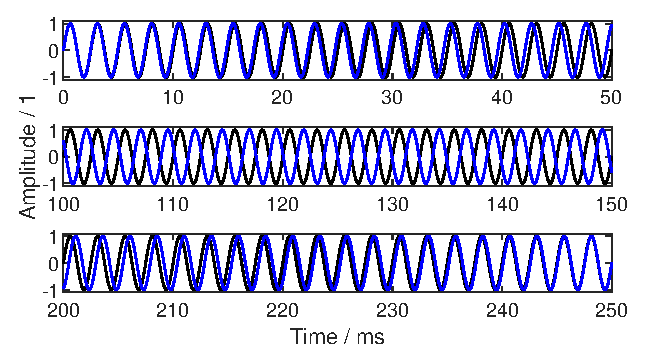
\includegraphics[width=\linewidth]{ue4/signal_beat.eps} % oder statt scale auch [width=0.5\textwidth] für eine feste Größe
  \caption{Darstellung der beiden Sinusschwingungen mit \SI{400}{\Hz} (schwarz) und \SI{404}{\Hz} (blau) während unterschiedlicher Phasenlagen. Im oberen Plot sieht man das langsame De-Phasing, der untere zeigt Re-Phasing. Im Mittleren hingegen wird die destruktive Interferenz in der maximalen Phasenverschiebung beider Signale gezeigt. Bei der Nullphase kann konstruktive Interferenz beobachtet werden.}
  \label{fig:signal}
\end{figure}

\begin{figure}[h]
\begin{subfigure}{.49\textwidth} 
  \centering
  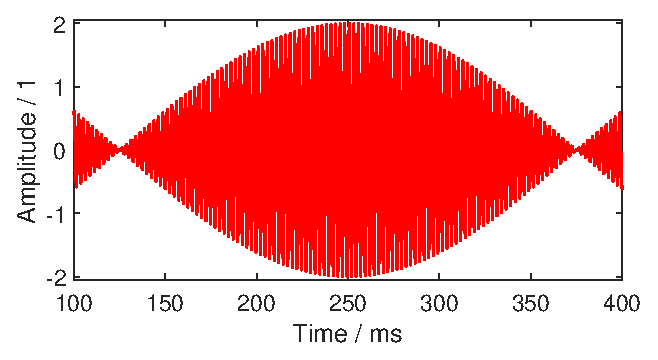
\includegraphics[width=\linewidth]{ue4/signaladdition.eps} % oder statt scale auch [width=0.5\textwidth] für eine feste Größe
  \caption{Die Überlagerung der \SI{400}{\Hz} und \SI{404}{\Hz} Töne resultiert in einem Signal, das einer Amplitudenmodulation gleicht.}
  \label{fig:signal_addition}
\end{subfigure}%
\hfill
\begin{subfigure}{.49\textwidth} 
  \centering
  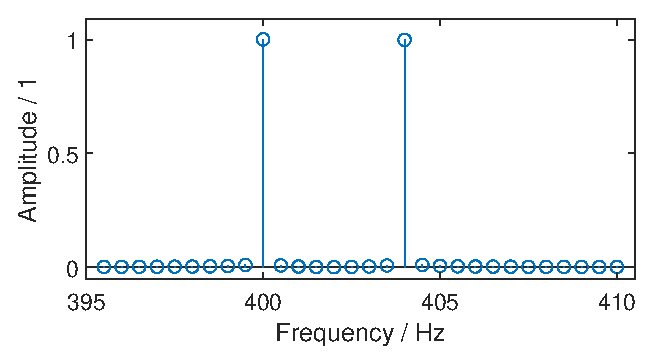
\includegraphics[width=\linewidth]{ue4/signaladdition_spectrum.eps} % oder statt scale auch [width=0.5\textwidth] für eine feste Größe
  \caption{Einseitiges Fourierspektrum des Superpositionssignals: Die beiden Überlagerungsfrequenzen sind klar unterscheidbar.}
  \label{fig:signal_fft}
\end{subfigure}
\caption{}
\label{fig:signal_super}
\end{figure}

\clearpage

\subsubsection{Amplitudenmodulation (AM)}
Bei der Amplitudenmodulation wird die Intensität eines konstanten Trägersignals mit einem zeitveränderlichen Signal verändert. Die Grundformel für diese Art der Datenübertragung zeigt Eq. \ref{eq:am}. Für das Ausgangssignal $y(t)$ wird das Signal traeger$(t)$ einerseits mit seiner spezifischen Amplitude $A$ und andererseits mit dem Modulationssignal modulator$(t)$ multipliziert und anschließend aufsummiert. 


\begin{align}
y(t)\ &=\ \left[A\ +\ \mathrm{modulator}(t) \right]\ \cdot\ \mathrm{traeger}(t) \label{eq:am} \\
    y(t) &= A (1\ +\ m\ \cdot\ \sin(\omega_M\ t))\ \cdot\ \sin(\omega_T\ t)\\
    \omega\ &=\ 2\pi f
\end{align}

In Figure \ref{fig:AM_1000_4} wurde ein Sinuston mit einer Trägerfrequenz $f_T$ von \SI{1000}{\Hz} mit einem Signal der Modulationsfrequenz $f_M =  \SI{4}{\Hz}$ unter dem Modulationsgrad $m =$ 0.5 beaufschlagt. Im einseitigen Amplitudenspektrum (Fig. \ref{fig:AM_1000_4_fft}) ist die Trägerfrequenz mit zwei, \SI{4}{\Hz}-entfernten Seitenbändern sichtbar. Durch den gewählten Modulationsfaktor besitzen diese eine Amplitude der viertelten Trägeramplitude, die zu eins gesetzt wurde. Diese Modulationsart nennt man nach der Anzahl der Seitenbänder \textit{Zwei-Seitenband-Modulation}.

\begin{figure}[h]
    \centering
\begin{subfigure}{.49\textwidth} 
  \centering
  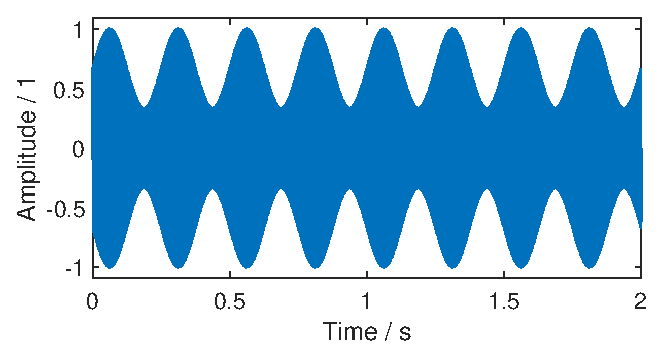
\includegraphics[width=.85\linewidth]{ue4/AM_1000_4.eps} % oder statt scale auch [width=0.5\textwidth] für eine feste Größe
  \caption{Amplitudenmodulierter Sinuston mit einer Trägerfrequenz $f_T$ von \SI{1000}{\Hz} und einem Signal der Modulationsfrequenz $f_M =  \SI{4}{\Hz}$ unter dem Modulationsgrad $m =$ 0.5.}
  \label{fig:AM_1000_4}
  \end{subfigure}%
\hfill
\begin{subfigure}{.49\textwidth} 
  \centering
  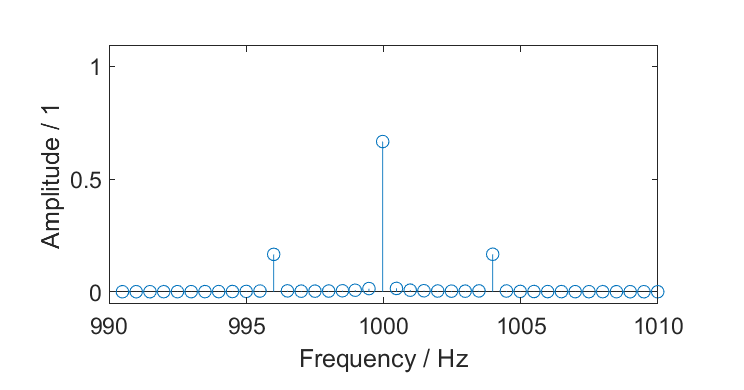
\includegraphics[width=\linewidth]{ue4/AM_1000_4_fft.eps} % oder statt scale auch [width=0.5\textwidth] für eine feste Größe
  \caption{Spektrum des AM-Signals aus Figure \ref{fig:AM_1000_4}. Die Trägerfrequenz und die beiden Seitenbänder im Abstand der Modulationsfrequenz sind klar sichtbar.}
  \label{fig:AM_1000_4_fft}
\end{subfigure}
    \caption{}
    \label{fig:AM}
\end{figure}
\clearpage

\subsubsection{Frequenzmodulation (FM)}


\begin{figure}[h]
    \centering
\begin{subfigure}{.49\textwidth} 
  \centering
  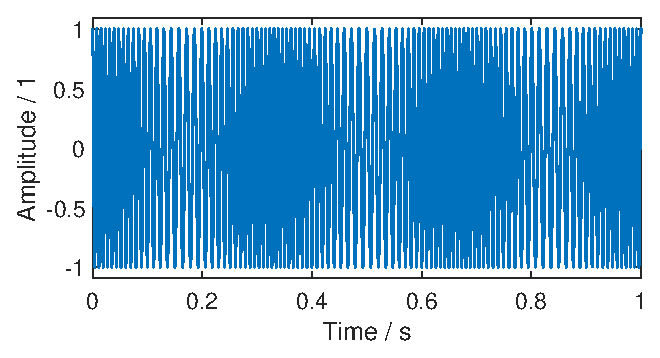
\includegraphics[width=.85\linewidth]{ue4/FM_100_3.eps} % oder statt scale auch [width=0.5\textwidth] für eine feste Größe
  \caption{FM-Signal mit den Parametern $f_T = \SI{100}{\Hz}$, $f_M = \SI{3}{\Hz}$ und $\Delta f_T = \SI{30}{\Hz}$.}
  \label{fig:FM_100_3}
  \end{subfigure}%
\hfill
\begin{subfigure}{.49\textwidth} 
  \centering
  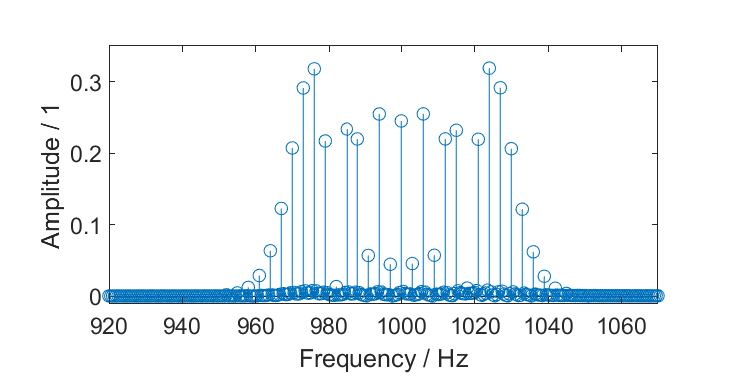
\includegraphics[width=\linewidth]{ue4/FM_1000_3_fft.eps} % oder statt scale auch [width=0.5\textwidth] für eine feste Größe
  \caption{Langzeitspektrum einer Schwingung mit den Parametern $f_T\ =\ \SI{1000}{\Hz}$, $f_M\ =\ \SI{3}{\Hz}$ und $\Delta f_T \SI{30}{\Hz}$.}
  \label{fig:FM_1000_3_fft}
\end{subfigure}
    \caption{}
    \label{fig:AM}
\end{figure}

Bei der Frequenzmodulation wird das Modulationssignal in den Frequenz-Phasenverlauf der Trägerschwingung hineinmoduliert. Ein resultierendes Signal mit den Parametern $f_T\ =\ \SI{100}{\Hz}$, $f_M\ =\ \SI{3}{\Hz}$ und einem Modulationshub $\Delta f_T$ von \SI{30}{\Hz} wurde zur leichteren Darstellung dieser Modulationsart in Figure \ref{fig:FM_100_3} geplottet. Das Signal berechnet sich nach folgender Formel, wobei $A_T$ und $A_M$ die Amplituden beider Sinusse bezeichnen.
\begin{equation}
    y(t) = A_T\ \cdot\ \cos\left(\omega_T\ t + \frac{\Delta f_T\ \cdot\ A_m}{f_M}\ \cdot\ \sin(\omega_M\ t)\right)
\end{equation}
Während des Anhörens eines ähnlichen Tons mit der Trägerfrequenz \SI{1000}{\Hz} konnte eine oszillierende Frequenz in Form einer Tonhöhenänderung wahrgenommen werden.

\begin{figure}[h]
    \centering
    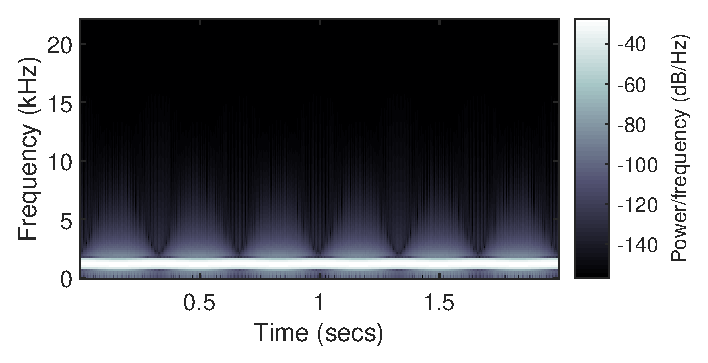
\includegraphics[width=.9\linewidth]{ue4/FM_1000_3_spect.eps}
    \caption{Spektrogramm eine Sinussignals mit $f_T\ =\ \SI{1000}{\Hz}$, $f_M\ =\ \SI{3}{\Hz}$ und $\Delta f_T\ =\  \SI{30}{\Hz}$. Der weiße Streifen zeigt die Trägerfrequenz, während die hellgrauen Hügel darüber die Frequenzen der überlagerten Besselfunktionen (der harmonischen Seitenschwingungen der Modulationsfrequenz) zeigen. Die Frequenz der Hüllkurve dieser Hügel ergibt sich zur Modulationsfrequenz.}
    \label{fig:FM_spectrogram}
\end{figure}

\clearpage

\subsubsection{Zu höheren Modulationsfrequenzen}
Analog zu Aufgabe 2 wurde diesmal ein Ton mit einer Modulationsfrequenz von $f_M\ =\ \SI{200}{\Hz}$ erzeugt.(Fig. \ref{fig:AM_1000_200}) Da die aufmodulierte Frequenz hier einen größeren Abstand zur Trägerfreqenz besitzt, ist der Einfluss der Interferenz auf das Signal nicht mehr hörbar. Dennoch hört man - möglicherweise durch Verdeckungseffekte des tiefen Seitenbandes bei \SI{800}{\Hz} (siehe Fig. \ref{fig:AM_1000_200_fft})  - die höheren Frequenzen leiser.

Durch bereits diskutierten Frequenzabstand sind die beiden bzw. drei Töne eindeutig voneinander unterscheidbar, was sich auf das Orts-Frequenzcoding der Cochlea zurückführen lässt. Bei zu naher Anregung zweier resonanter Regionen auf der Basilarmembran durch die Wanderwelle, verschwimmen die Töne zu einem oder nur der tiefere ist durch den Verdeckungseffekt zu hören.
\begin{figure}[h]
    \centering
\begin{subfigure}{.49\textwidth} 
  \centering
  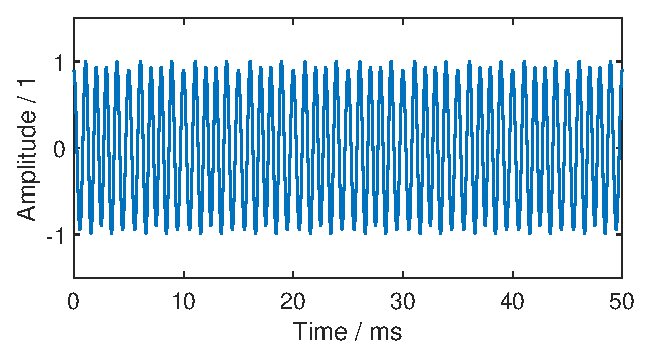
\includegraphics[width=.9\linewidth]{ue4/AM_1000_200.eps} % oder statt scale auch [width=0.5\textwidth] für eine feste Größe
  \caption{AM-Signal mit einer Trägerfrequenz $f_T$ von \SI{1000}{\Hz} und einem Signal der Modulationsfrequenz $f_M =  \SI{200}{\Hz}$ unter dem Modulationsgrad $m =$ 0.5.}
  \label{fig:AM_1000_200}
  \end{subfigure}%
\hfill
\begin{subfigure}{.49\textwidth} 
  \centering
  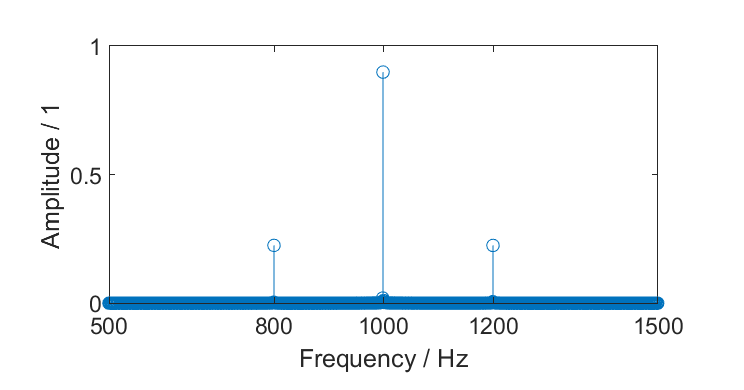
\includegraphics[width=\linewidth]{ue4/AM_1000_200_fft.eps} % oder statt scale auch [width=0.5\textwidth] für eine feste Größe
  \caption{Spektrum des AM-Signals aus Figure \ref{fig:AM_1000_200}. Die Trägerfrequenz und die beiden Seitenbänder im Abstand der Modulationsfrequenz sind klar sichtbar.}
  \label{fig:AM_1000_200_fft}
\end{subfigure}
    \caption{}
    \label{fig:AM_1000_200_fig}
\end{figure}


\subsubsection{Freiwillige Fleißaufgabe}
Es wurden drei Sinustöne mit den Frequenzen $f\ =\ $ \SIlist[list-final-separator={ ,und }]{400;400.25;500}{\Hz} generiert, um eine akustische Sinnestäuschung zu erzeugen. Zusätzlich wurden diese Signale mit $f_M\ =\ \SI{5}{\Hz}$ unter dem Modulationsgrad $m\ =\ 1$ amplitudenmoduliert. Bei einem Abspielen der Kombinationen 400/\SI{500}{\Hz} und 400/\SI{400.25}{\Hz} in jeweils einem Stereokanal der Kopfhörer entsteht die Illusion eines Tones zwischen beiden Frequenzen, der mit der Differenz beider Äußerer lauter und leiser wird; ein sogenannter binauraler Beat. In der letzteren Kombination ist der Intensitätsunterschied sehr deutlich hörbar.

Da beide Töne in unterschiedlichen Ohren ankommen, muss der Sinneseindruck im Gehirn an einer Stelle stattfinden, in der beide Signale gleichsam eintreffen. Die ersten Stellen, an denen diese Möglichkeit bestünde, wäre der Colliculus inferior oder die obere Olive. Dort vermuten Forscher derzeit auch die Entstehung dieses Phänomens.




\clearpage